\documentclass[11pt]{article}
\usepackage[T1]{fontenc}
\usepackage[utf8]{inputenc}
\usepackage{graphicx}
\usepackage[french]{babel}
\usepackage[right=2.5cm, bottom=2.5cm,top=2.5cm, left=2.5cm]{geometry}
\title{\vspace{\fill} Interface et Multimédia \\ ~\textbf{IFT-215} \\~\\ Travail Pratique 4}
\author{Amandine Fouillet - 14 130 638 ~\\ Frank Chassing - 14 153 710 ~\\ Laurent Sénécal-Léonard - 14 143 484}
\date{\today \vspace{\fill}}

\begin{document}
\maketitle
\newpage \thispagestyle{empty}
\null
\newpage
\tableofcontents

\newpage
\section*{Introduction \markboth{INTRODUCTION}{}}
\addcontentsline{toc}{section}{Introduction}
Après avoir étudié les différents acteurs, analysé leurs différents environnements et détaillé l’ensemble des fonctionnalités que nous voulons voir apparaître dans notre application, nous exposerons dans ce rapport l’ensemble des modélisations de nos données par le biais de diagrammes UML. Pour cela, nous commencerons par décrire les  diagrammes de nos fonctionnalités en identifiant les différents attributs et les différentes méthodes liés à celles-ci. Puis nous effectuerons un compte rendu global de notre diagramme afin d’observer les différents liens entre nos classes.

\section{Modélisation de la gestion de la Communication}
\begin{figure}[!h]
        \centering 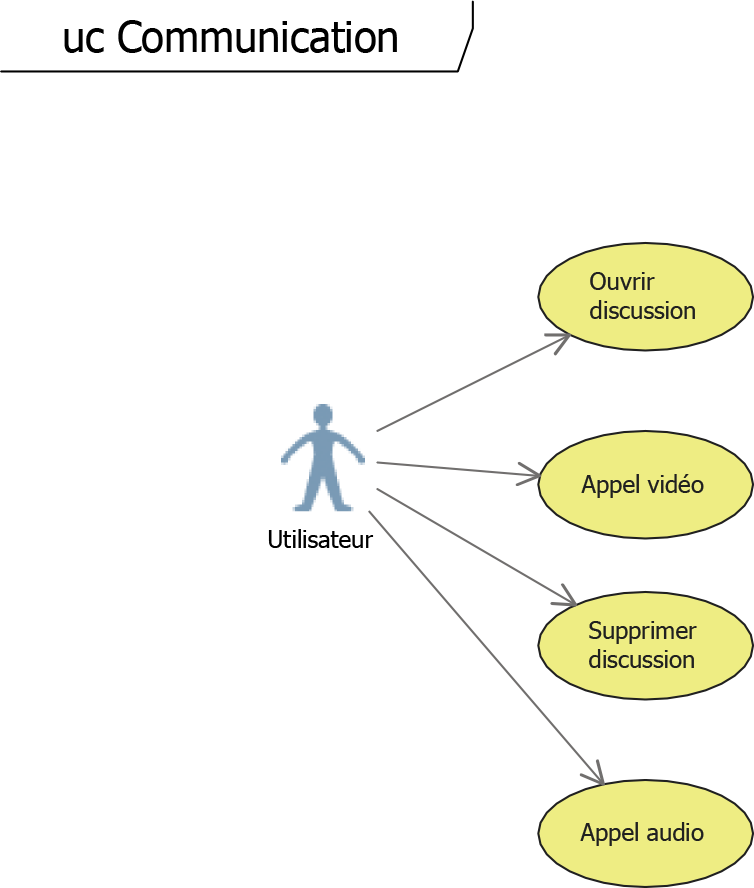
\includegraphics[scale=1]{ucCom.png}
        \caption{Cas d'utilisation communication}
         \label{fig:ucCom}
\end{figure}
\begin{figure}[!h]
        \centering 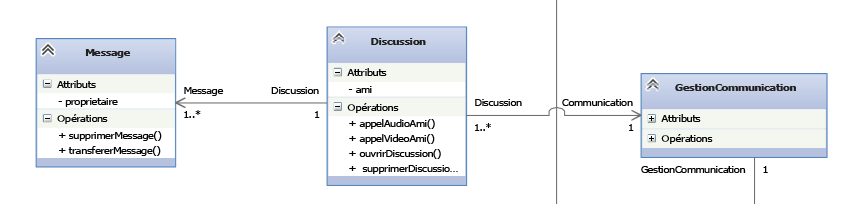
\includegraphics[scale=1]{com.png}
        \caption{Diagramme de classe communication}
         \label{fig:com}
\end{figure}

\newpage
\section{Modélisation de la gestion des Photos}
\begin{figure}[!h]
        \centering 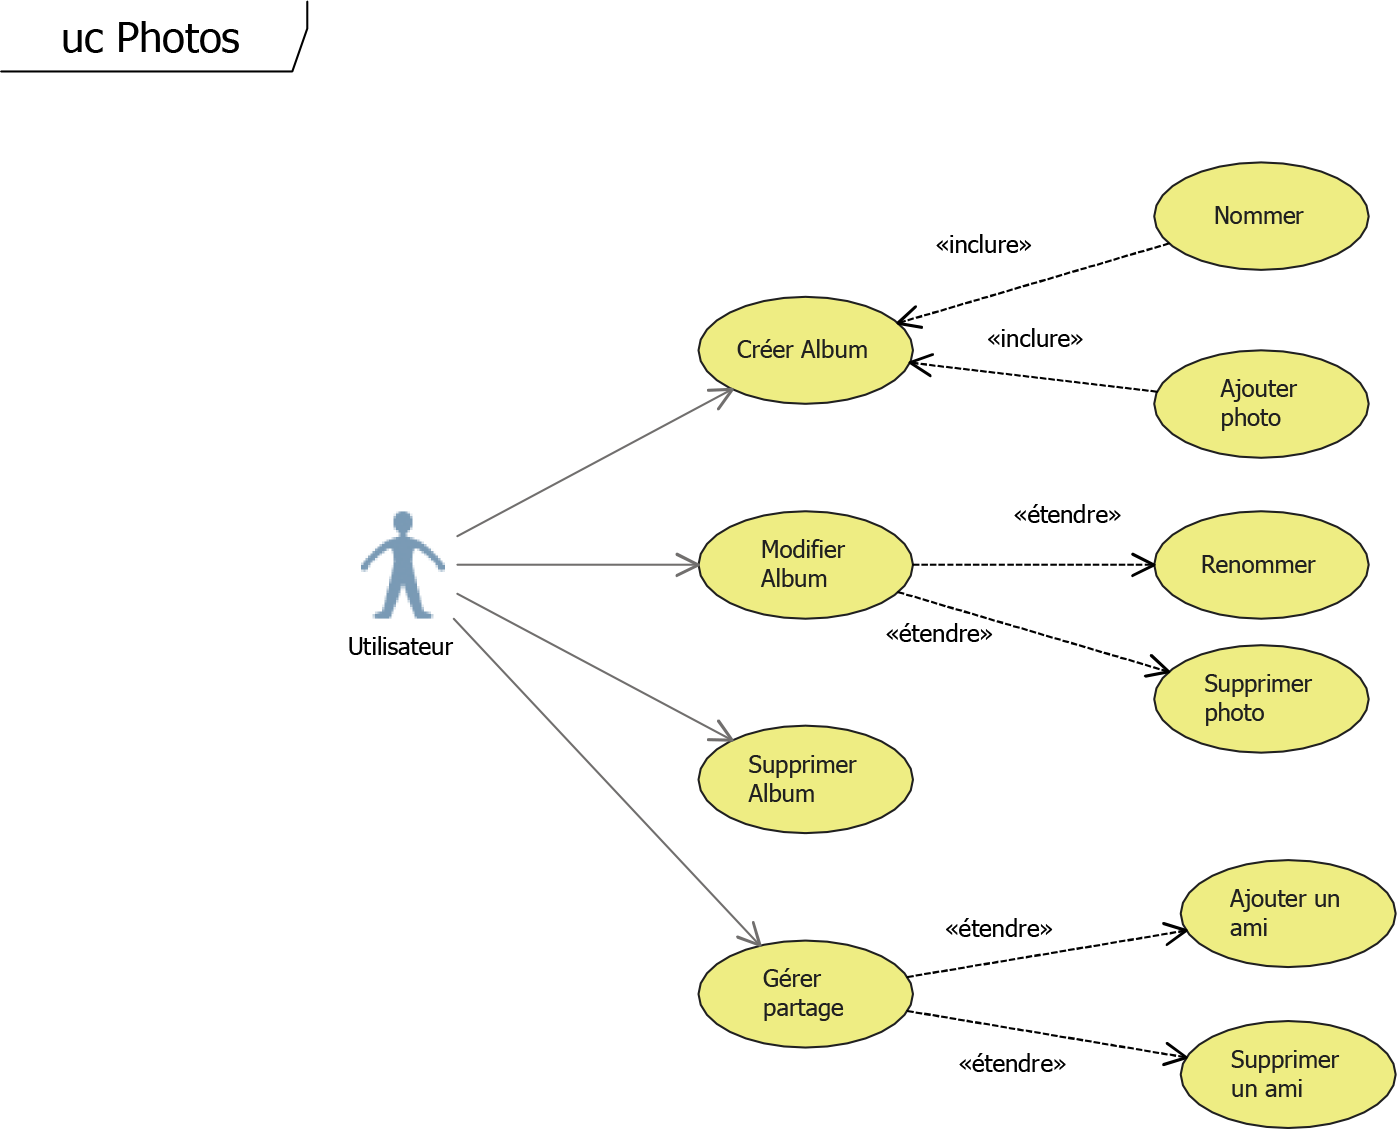
\includegraphics[scale=1]{ucPhotos.png}
        \caption{Cas d'utilisation photos}
         \label{fig:ucPhotos}
\end{figure}
\begin{figure}[!h]
        \centering 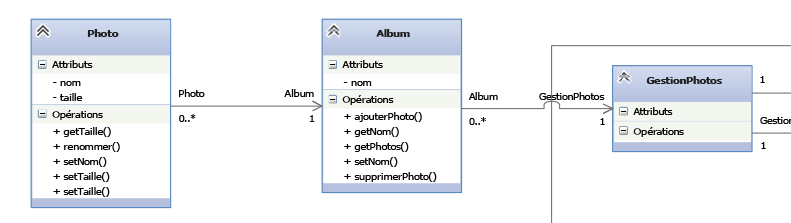
\includegraphics[scale=1]{photo.png}
        \caption{Diagramme de classe photos}
         \label{fig:photos}
\end{figure}

\newpage
\section{Modélisation de la gestion du Calendrier}
\begin{figure}[!h]
        \centering 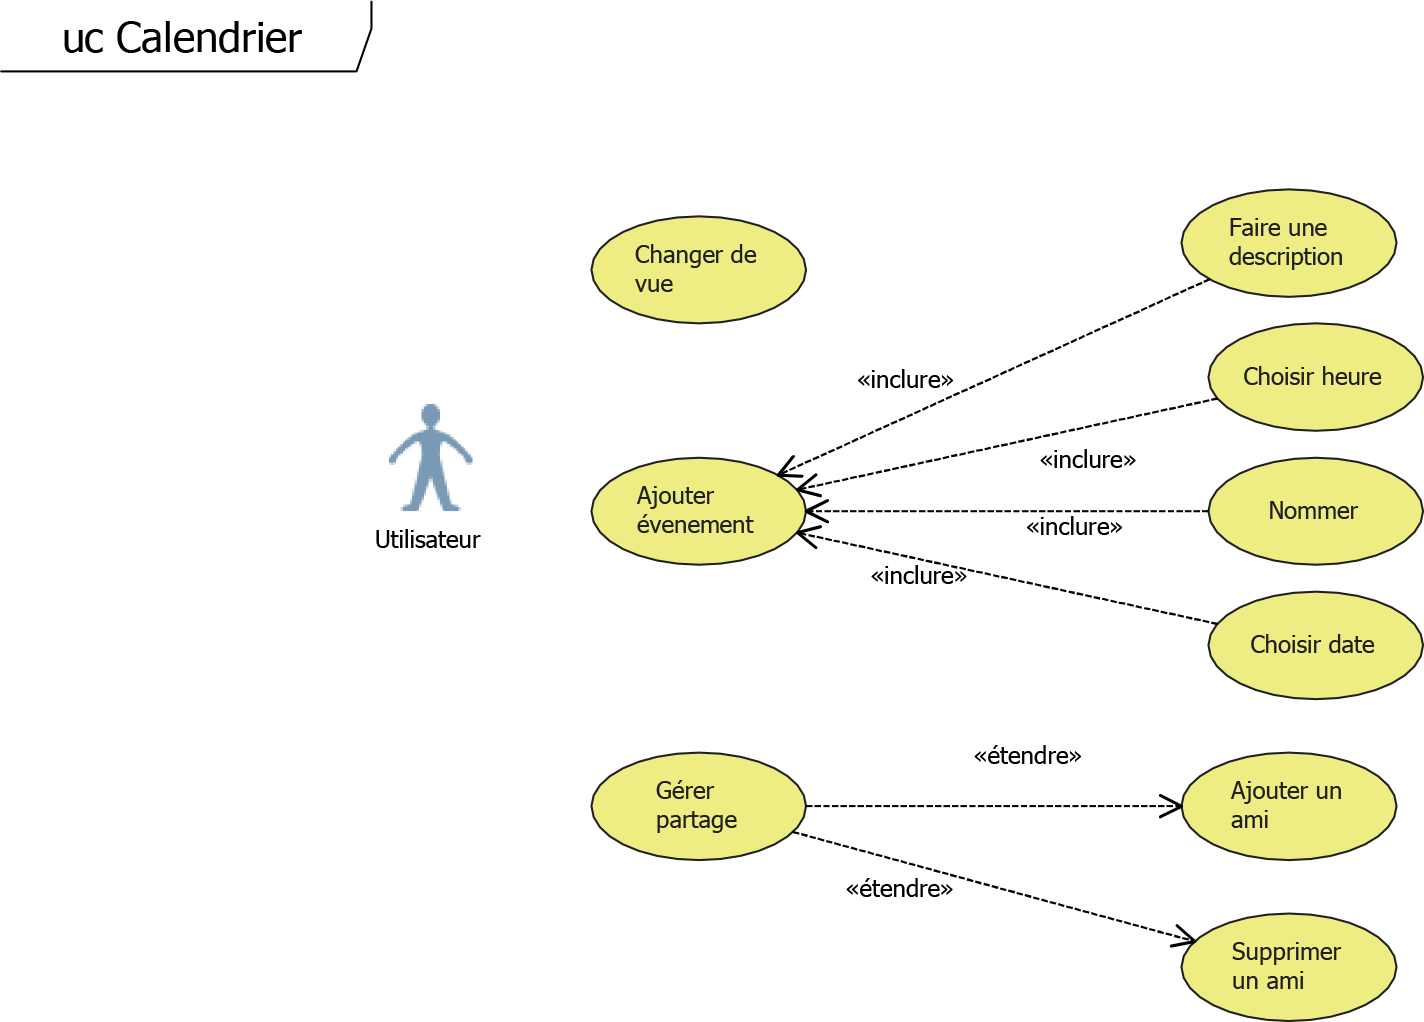
\includegraphics[scale=1]{ucCal.png}
        \caption{Cas d'utilisation calendrier}
         \label{fig:ucCal}
\end{figure}
\begin{figure}[!h]
        \centering 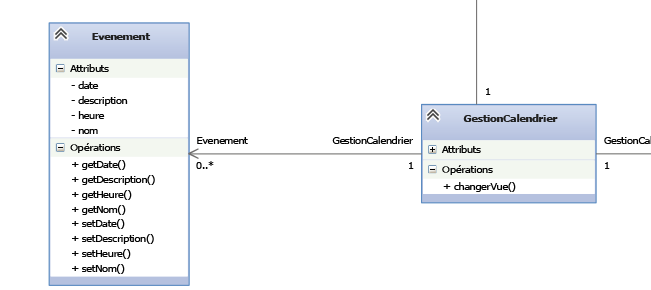
\includegraphics[scale=1]{calendrier.png}
        \caption{Diagramme de classe calendrier}
         \label{fig:cal}
\end{figure}

\newpage
\section{Modélisation de la gestion des Dépenses}
\begin{figure}[!h]
        \centering 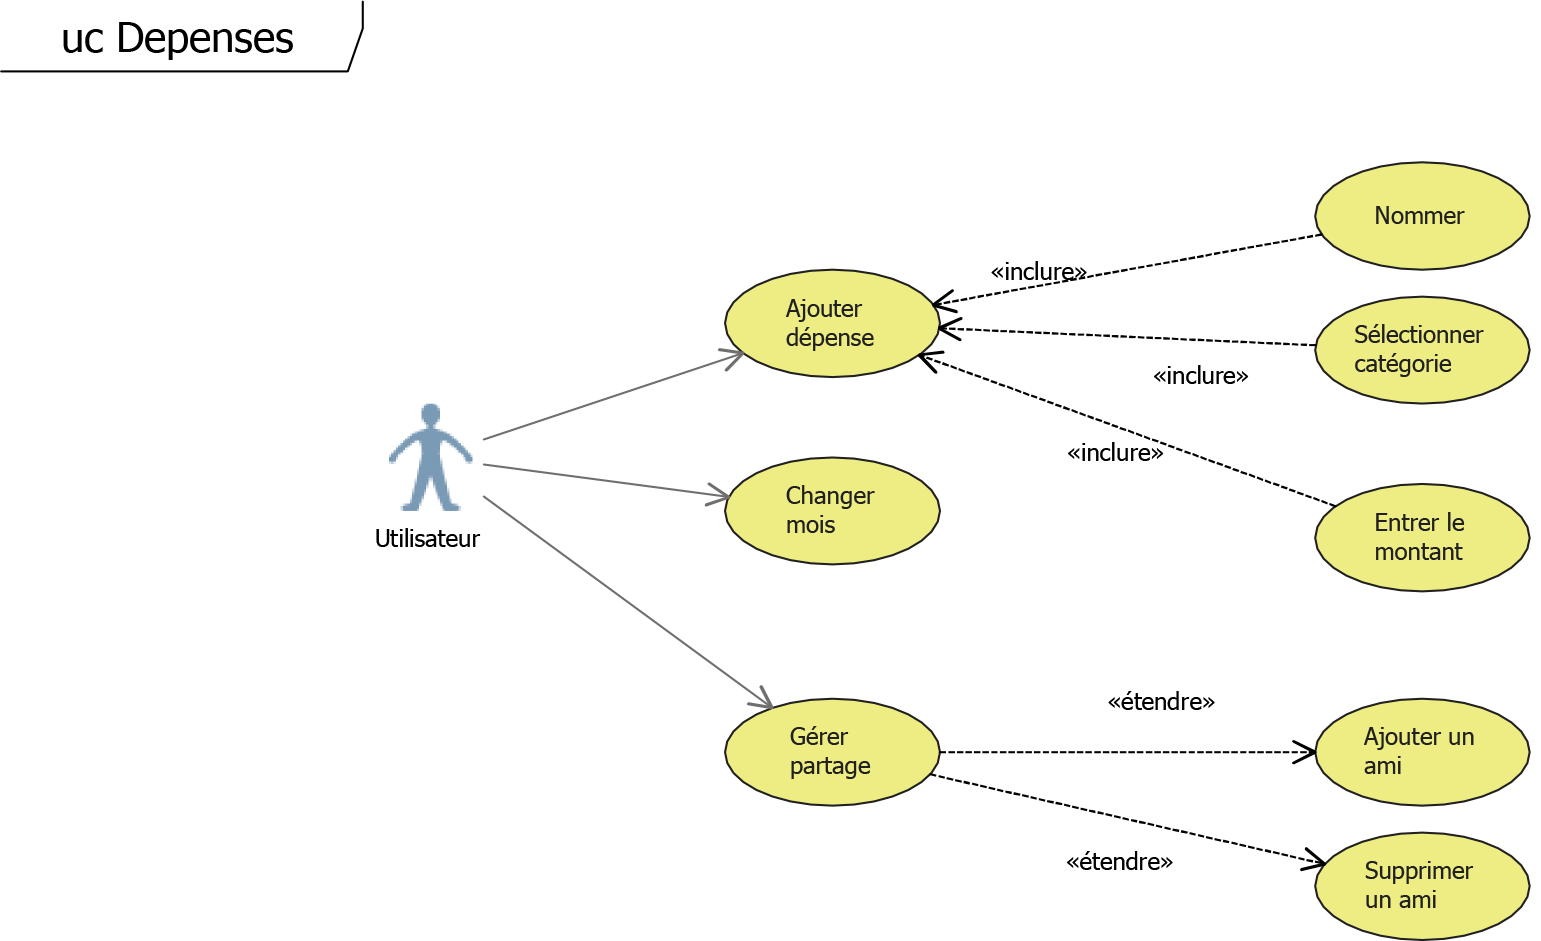
\includegraphics[scale=1]{ucDepenses.png}
        \caption{Cas d'utilisation dépenses}
         \label{fig:ucDepenses}
\end{figure}
\begin{figure}[!h]
        \centering 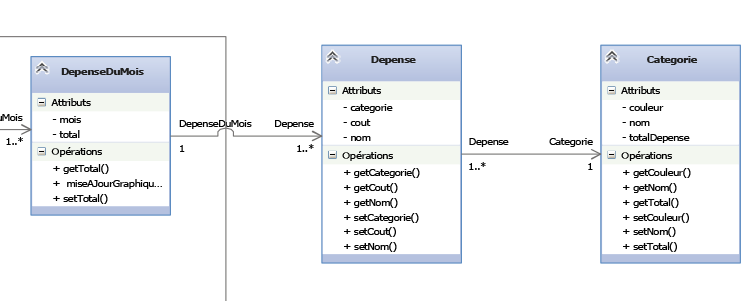
\includegraphics[scale=1]{depense.png}
        \caption{Diagramme de classe dépenses}
         \label{fig:depense}
\end{figure}!h

\newpage
\section{Modélisation de la gestion de la Carte}
\begin{figure}[!h]
        \centering 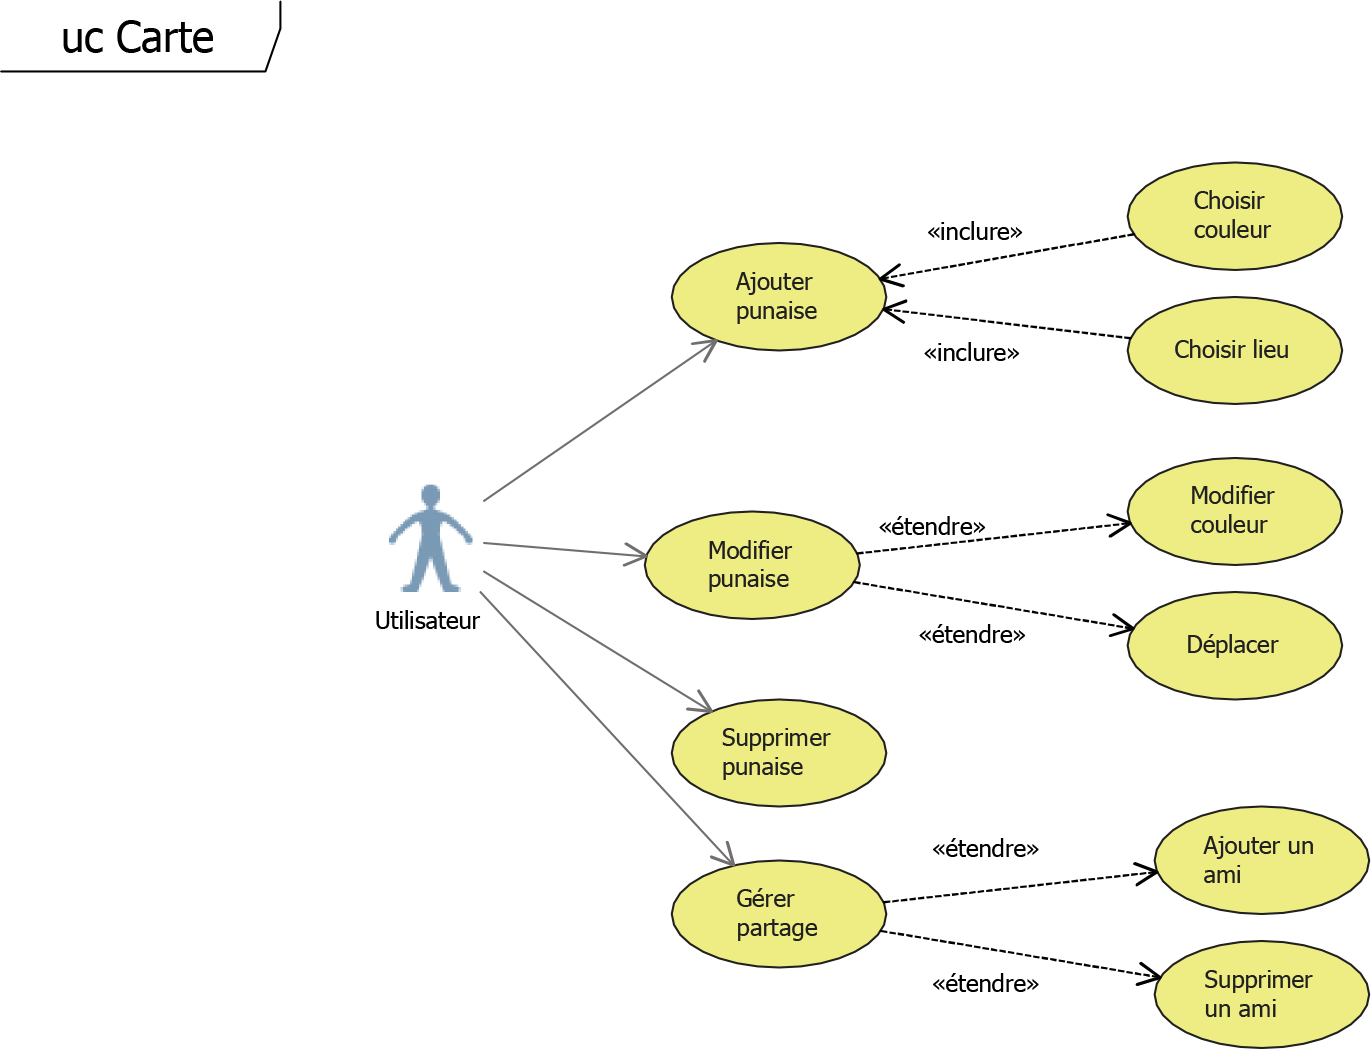
\includegraphics[scale=1]{ucCarte.png}
        \caption{Cas d'utilisation carte}
         \label{fig:ucCarte}
\end{figure}
Le diagramme de cas d’utilisation  (\textsc{Figure \ref{fig:ucCarte}}) permet de nous rappeler les différentes fonctionnalités que peut exécuter l’utilisateur dans cette section. Celui-ci pourra à tout moment ajouter une punaise sur la carte du monde afin de dire qu’il a voyagé à l’endroit où se situe la punaise. Il pourra bien évidemment déplacer ou bien supprimer sa punaise. Il pourra également modifier la couleur de celle-ci pour créer des groupes ou des jeux de couleur.
\begin{figure}[!h]
        \centering 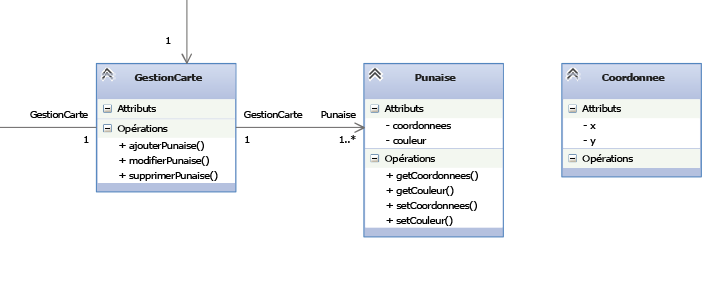
\includegraphics[scale=1]{carte.png}
        \caption{Diagramme de classe carte}
         \label{fig:carte}
\end{figure}
Au niveau du diagramme de classe  (\textsc{Figure \ref{fig:carte}}), nous aurons une classe permettant la gestion de la carte qui contiendra une ou plusieurs punaises ainsi que les différentes actions sur les punaises (ajouter, modifier, supprimer). La classe Punaise, quant à elle, permet de modéliser une punaise. Elle possède donc comme attribut les coordonnées de la punaise, sa couleur et une description permettant à l'utilisateur de raconter les joies de ses voyages. En ce qui concerne les méthodes, nous retrouvons les différents accesseurs (get et set) permettant de récupérer ou modifier les attributs. Nous avons également ajouté une classe Coordonnées avec une position x et y en attribut représentant respectivement l’abscisse et l’ordonnée.
\newpage
\section{Modélisation de la gestion des Contacts}
\begin{figure}[!h]
        \centering 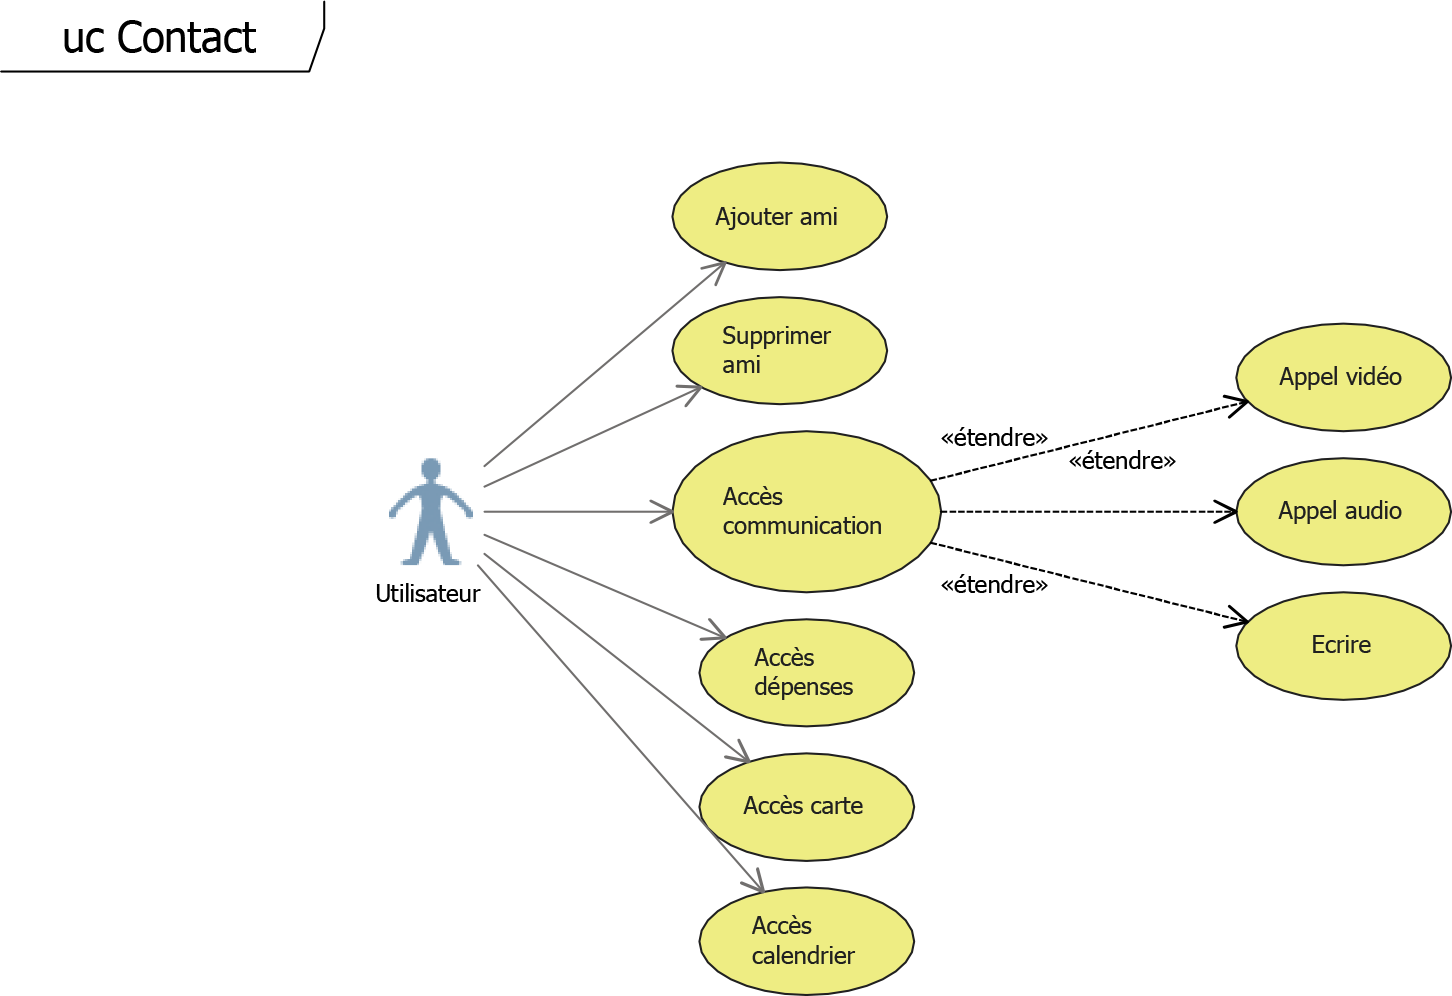
\includegraphics[scale=1]{ucContact.png}
        \caption{Cas d'utilisation contacts}
         \label{fig:ucContact}
\end{figure}
\begin{figure}[!h]
        \centering 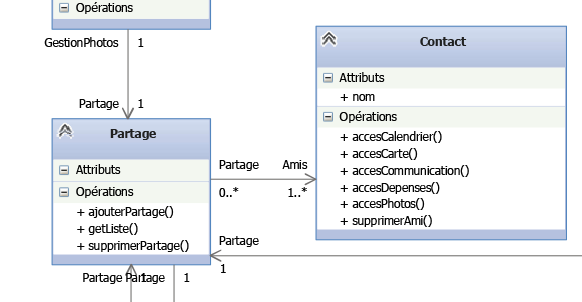
\includegraphics[scale=1]{contact.png}
        \caption{Diagramme de classe contact}
         \label{fig:contact}
\end{figure}
Nous retrouvons encore ici un diagramme de cas d’utilisation  (\textsc{Figure \ref{fig:ucContact}})modélisant les fonctionnalités de la section Contacts. L’utilisateur sera en mesure d’ajouter ou bien supprimer un contact à tout moment. Il pourra également observer les différentes informations sur le contact telles que ses dépenses, sa carte du monde, ses photos ou son emploi du temps. L’utilisateur aura également un accès pour communiquer avec le contact soit par vidéo, audio ou chat.
La modélisation des données est représentée par une seule classe « Contact »  (\textsc{Figure \ref{fig:contact}}). Chaque contact sera un objet de cette classe et possèdera des paramètres correspondant à ses informations personnelles telles que son nom, son prénom, son numéro, son mail ou encore son adresse. Pour chaque contact, l’utilisateur a un accès pour chaque information de celui-ci telle que son calendrier, sa carte ou son emploi du temps et un accès pour communiquer avec lui. C’est pourquoi nous retrouvons les différentes méthodes d’accès : accesCalendrier(), accesCarte(), accesCommunication(), accesDepense() et accesPhoto(). Ces méthodes donneront l’accès à l’utilisateur aux différentes sections. L’utilisateur aura également la possibilité de supprimer le contact grâce à la méthode supprimerContact().


\newpage
\section{Diagramme de classe global}
\begin{figure}[!h]
        \centering 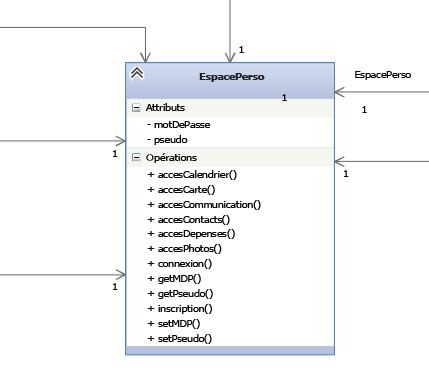
\includegraphics[scale=2]{espace.png}
        \caption{Diagramme de classe espace personnel}
         \label{fig:espace}
\end{figure}

La classe EspacePerso (\textsc{Figure \ref{fig:espace}}) est la classe qui va permettre de gérer le compte utilisateur ainsi que toutes ses données. Cette classe a deux attributs privés : le pseudo et le mot de passe qui permettent de retrouver et reconnaitre l'utilisateur. Elle contient des méthodes d'accès (get et set) pour récupérer ou modifier ses attributs. Les méthodes publiques inscription() et connexion() permettent respectivement de gérer la création de l'espace personnel et l'accès à cet espace. On retrouve ensuite toutes les méthodes d'accès au différentes données de l'utilisateur : ses contacts, sa carte, son calendrier, ses dépenses, ses communications et ses photos. 


\begin{figure}[!h]
        \centering 
\includegraphics[scale=2]{partage.png}
        \caption{Diagramme de classe partage}
         \label{fig:partage}
\end{figure}

La classe Partage (\textsc{Figure \ref{fig:partage}}) est la classe qui va permettre à l'utilisateur de gérer les listes de contacts avec qui il veut partager ses différentes informations. 
Pour rappel, dans notre application, il sera possible à l'utilisateur de partager ses photos, son calendrier, sa carte ainsi que ses dépenses. Il nous semble important de laisser la possibilité à l'utilisateur de créer des listes de partage différentes afin de lui laisser la possibilité de ne pas tout partager aux mêmes personnes. Par exemple un étudiant peut décider de partager ses dépenses seulement avec ses parents et ses photos de soirée seulement avec ses amis. 
Pour implémenter cela, nous avons décidé de créer la classe Partage qui sera finalement qu'une sorte de liste améliorée de contacts. Pour chacune des catégories (carte, dépenses, photos et calendrier) un partage sera créé et grâce aux méthodes ajouterPartage() et supprimerPartage() il sera possible d'ajouter ou de supprimer des contacts à qui l'accès à la catégorie sera autorisé.

\newpage
\begin{figure}[!h]
        \centering 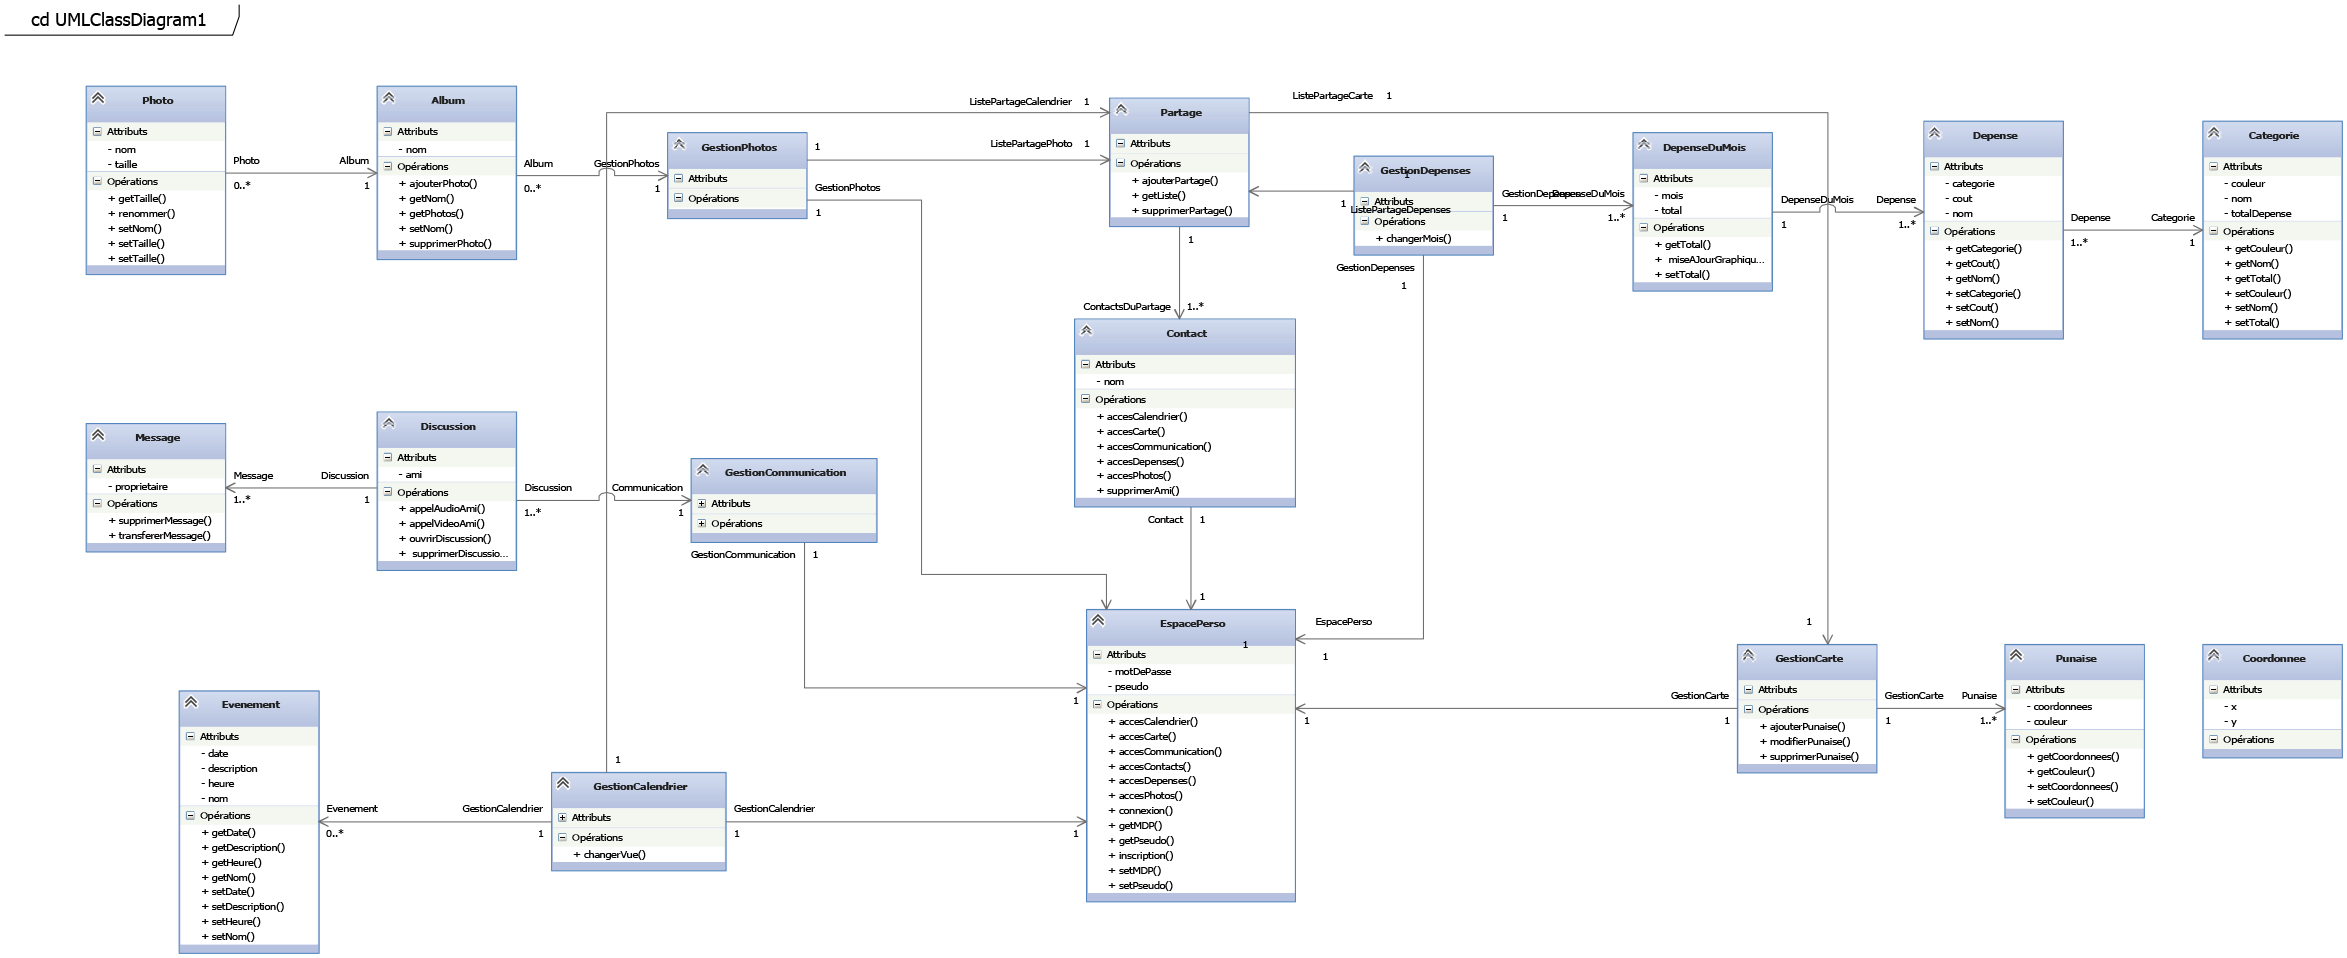
\includegraphics[scale=0.9]{classe.png}
        \caption{Diagramme de classe}
         \label{fig:classe}
\end{figure}

La \textsc{Figure \ref{fig:classe}} représente le diagramme de classe de l'application dans sa globalité. On retrouve les différentes classes que l'on a détaillées et expliquées précédement. On peut cependant constater les dépendances et les relations entre ces différentes classes : 
\begin{itemize}
\item la classe EspacePerso est reliée avec les classes GestionPhotos, GestionCommunication, GestionCarte, GestionDépenses, Contact et GestionCalendrier. Cela est dû au fait que chaque espace personnel d'un utilisateur est constitué de chacun des espaces précédemment cités. Cette modélisation nous permet de séparer les différentes catégories et de gérer les différents écrans dans l'interface. En effet, chaque espace personnel sera composé d'une liste de contacts et de plusieurs zones où l'utilisateur pourra gérer ses informations.
\item la classe Partage est reliée avec les classes GestionPhotos, GestionCarte, GestionDépenses et GestionCalendrier. En effet, ce sont les quatre espaces qui peuvent être partagés avec les contacts de l'utilisateur. Elle est aussi reliée à la classe Contact car c'est une classe étant donné qu'elle est constituée de plusieurs contacts.
\end{itemize}

\section*{Conclusion \markboth{CONCLUSION}{}}
\addcontentsline{toc}{section}{Conclusion}
Ce quatrième rapport consiste en la modélisation de nos données, ce qui correspond au M du modèle MVC. La modélisation UML dans ce rapport permet de créer un squelette d’implémentation qui nous aide à avoir une bonne base de code ayant du sens. Chaque classe à une fonction précise et possède de nombreux paramètres caractérisant celle-ci. Elle contient également plusieurs méthodes permettant de gérer plusieurs évènements et plusieurs actions liées à la classe. Chaque liaison entre les classes ont un sens et prennent soin d’apporter de la concordance entre les classes. Le modèle MVC permet notamment d’observer la manipulation des données et le traitement de celles-ci. Dans le prochain TP, nous mettrons en place un premier prototype fonctionnel  de notre application afin de pouvoir le présenter oralement.
\newpage
\listoffigures


\end{document}